\documentclass{standalone}
\usepackage{tikz}
\usetikzlibrary{patterns, positioning}

\begin{document}
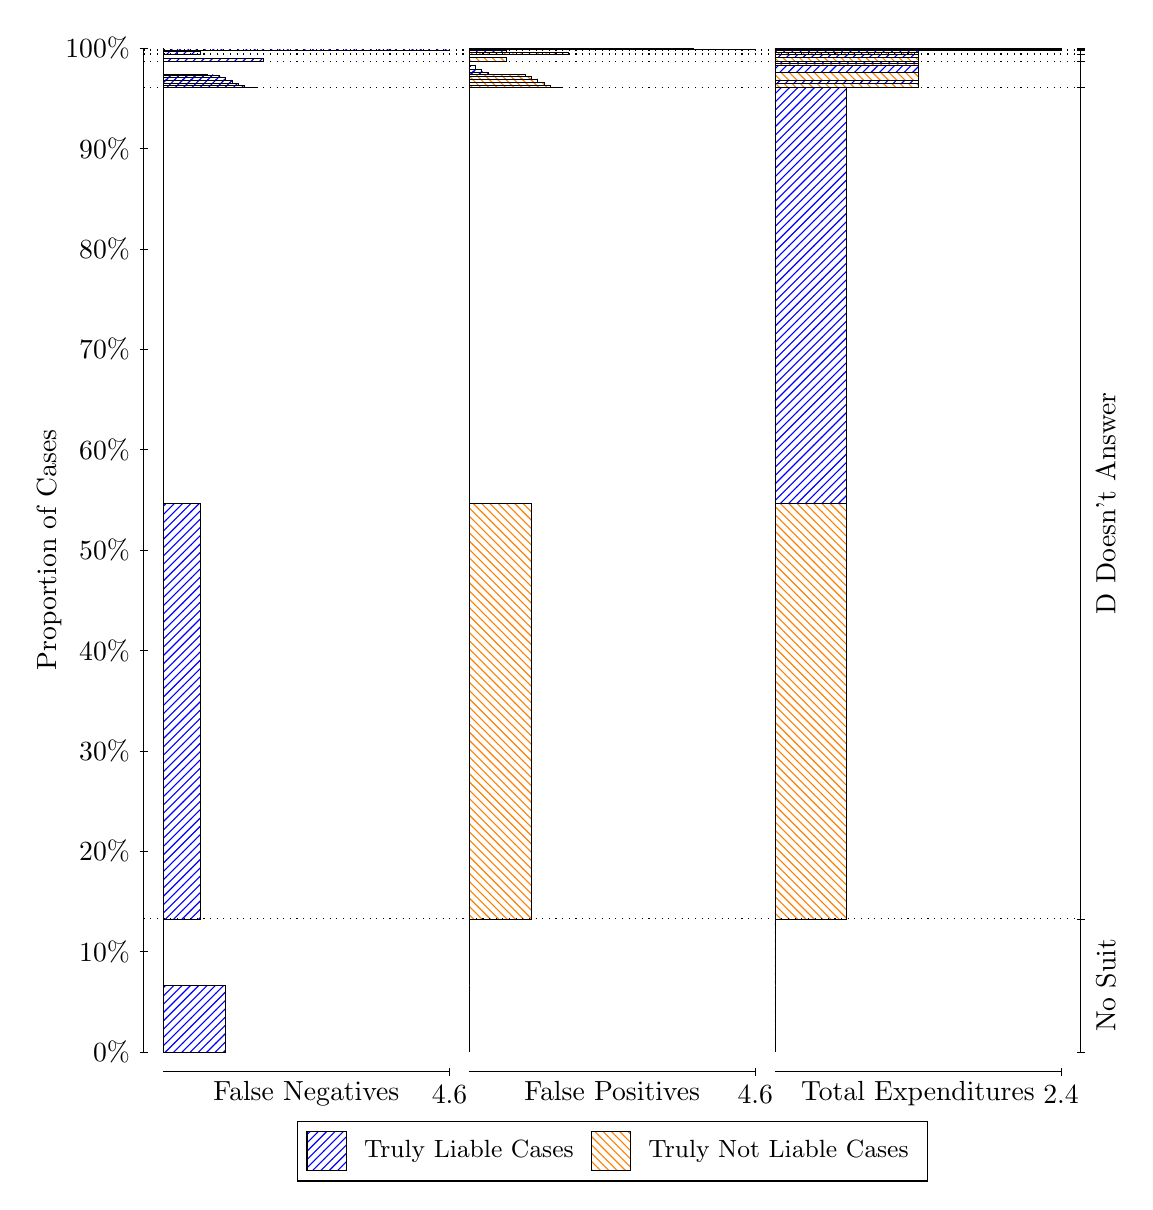
\begin{tikzpicture}
\draw[black, very thin] (1.5,1.75) -- (1.5,14.5);
\node[rotate=90, anchor=center] at (0.3, 8.125) {Proportion of Cases};
\draw[black, very thin] (1.45,1.75) -- (1.55,1.75);
\node[anchor=east] at (1.45, 1.75) {0\%};
\draw[black, very thin] (1.45,3.025) -- (1.55,3.025);
\node[anchor=east] at (1.45, 3.025) {10\%};
\draw[black, very thin] (1.45,4.3) -- (1.55,4.3);
\node[anchor=east] at (1.45, 4.3) {20\%};
\draw[black, very thin] (1.45,5.575) -- (1.55,5.575);
\node[anchor=east] at (1.45, 5.575) {30\%};
\draw[black, very thin] (1.45,6.85) -- (1.55,6.85);
\node[anchor=east] at (1.45, 6.85) {40\%};
\draw[black, very thin] (1.45,8.125) -- (1.55,8.125);
\node[anchor=east] at (1.45, 8.125) {50\%};
\draw[black, very thin] (1.45,9.4) -- (1.55,9.4);
\node[anchor=east] at (1.45, 9.4) {60\%};
\draw[black, very thin] (1.45,10.675) -- (1.55,10.675);
\node[anchor=east] at (1.45, 10.675) {70\%};
\draw[black, very thin] (1.45,11.95) -- (1.55,11.95);
\node[anchor=east] at (1.45, 11.95) {80\%};
\draw[black, very thin] (1.45,13.225) -- (1.55,13.225);
\node[anchor=east] at (1.45, 13.225) {90\%};
\draw[black, very thin] (1.45,14.5) -- (1.55,14.5);
\node[anchor=east] at (1.45, 14.5) {100\%};

\draw[black, very thin] (13.4,1.75) -- (13.4,14.5);
\draw[black, very thin] (13.35,1.75) -- (13.45,1.75);
\node[anchor=west] at (13.35, 1.75) {};
\draw[black, very thin] (13.35,3.4407) -- (13.45,3.4407);
\node[anchor=west] at (13.35, 3.4407) {};
\draw[black, very thin] (13.35,14) -- (13.45,14);
\node[anchor=west] at (13.35, 14) {};
\draw[black, very thin] (13.35,14.328) -- (13.45,14.328);
\node[anchor=west] at (13.35, 14.328) {};
\draw[black, very thin] (13.35,14.424) -- (13.45,14.424);
\node[anchor=west] at (13.35, 14.424) {};
\draw[black, very thin] (13.35,14.474) -- (13.45,14.474);
\node[anchor=west] at (13.35, 14.474) {};
\draw[black, very thin] (13.35,14.478) -- (13.45,14.478);
\node[anchor=west] at (13.35, 14.478) {};
\draw[black, very thin] (13.35,14.5) -- (13.45,14.5);
\node[anchor=west] at (13.35, 14.5) {};

\draw[black, very thin, pattern color=blue, pattern=north east lines] (1.75,1.75) rectangle (2.5399,2.5953);
\draw[black, very thin, pattern color=orange, pattern=north west lines] (1.75,2.5953) rectangle (1.75,3.4407);
\draw[black, very thin, pattern color=blue, pattern=north east lines] (1.75,3.4407) rectangle (2.2239,8.7189);
\draw[black, very thin, pattern color=orange, pattern=north west lines] (1.75,8.7189) rectangle (1.75,14);
\draw[black, very thin, pattern color=blue, pattern=north east lines] (1.75,14) rectangle (2.9348,14.003);
\draw[black, very thin, pattern color=blue, pattern=north east lines] (1.75,14.003) rectangle (2.8558,14.005);
\draw[black, very thin, pattern color=blue, pattern=north east lines] (1.75,14.005) rectangle (2.7768,14.026);
\draw[black, very thin, pattern color=blue, pattern=north east lines] (1.75,14.026) rectangle (2.6978,14.05);
\draw[black, very thin, pattern color=blue, pattern=north east lines] (1.75,14.05) rectangle (2.6188,14.095);
\draw[black, very thin, pattern color=blue, pattern=north east lines] (1.75,14.095) rectangle (2.5399,14.133);
\draw[black, very thin, pattern color=blue, pattern=north east lines] (1.75,14.133) rectangle (2.4609,14.156);
\draw[black, very thin, pattern color=blue, pattern=north east lines] (1.75,14.156) rectangle (2.3819,14.16);
\draw[black, very thin, pattern color=blue, pattern=north east lines] (1.75,14.16) rectangle (2.3029,14.162);
\draw[black, very thin, pattern color=orange, pattern=north west lines] (1.75,14.162) rectangle (1.75,14.328);
\draw[black, very thin, pattern color=blue, pattern=north east lines] (1.75,14.328) rectangle (3.0138,14.367);
\draw[black, very thin, pattern color=orange, pattern=north west lines] (1.75,14.367) rectangle (1.75,14.424);
\draw[black, very thin, pattern color=blue, pattern=north east lines] (1.75,14.424) rectangle (2.2239,14.453);
\draw[black, very thin, pattern color=orange, pattern=north west lines] (1.75,14.453) rectangle (1.75,14.474);
\draw[black, very thin, pattern color=blue, pattern=north east lines] (1.75,14.474) rectangle (5.3833,14.475);
\draw[black, very thin, pattern color=orange, pattern=north west lines] (1.75,14.475) rectangle (1.75,14.478);
\draw[black, very thin, pattern color=orange, pattern=north west lines] (1.75,14.478) rectangle (1.75,14.479);
\draw[black, very thin, pattern color=blue, pattern=north east lines] (1.75,14.479) rectangle (1.75,14.5);
\draw[black, very thin, pattern color=orange, pattern=north west lines] (5.6333,1.75) rectangle (5.6333,2.5953);
\draw[black, very thin, pattern color=blue, pattern=north east lines] (5.6333,2.5953) rectangle (5.6333,3.4407);
\draw[black, very thin, pattern color=orange, pattern=north west lines] (5.6333,3.4407) rectangle (6.4232,8.7219);
\draw[black, very thin, pattern color=blue, pattern=north east lines] (5.6333,8.7219) rectangle (5.6333,14);
\draw[black, very thin, pattern color=orange, pattern=north west lines] (5.6333,14) rectangle (6.8181,14.002);
\draw[black, very thin, pattern color=orange, pattern=north west lines] (5.6333,14.002) rectangle (6.7391,14.004);
\draw[black, very thin, pattern color=orange, pattern=north west lines] (5.6333,14.004) rectangle (6.6601,14.024);
\draw[black, very thin, pattern color=orange, pattern=north west lines] (5.6333,14.024) rectangle (6.5812,14.063);
\draw[black, very thin, pattern color=orange, pattern=north west lines] (5.6333,14.063) rectangle (6.5022,14.109);
\draw[black, very thin, pattern color=orange, pattern=north west lines] (5.6333,14.109) rectangle (6.4232,14.138);
\draw[black, very thin, pattern color=orange, pattern=north west lines] (5.6333,14.138) rectangle (6.3442,14.162);
\draw[black, very thin, pattern color=orange, pattern=north west lines] (5.6333,14.162) rectangle (6.2652,14.164);
\draw[black, very thin, pattern color=orange, pattern=north west lines] (5.6333,14.164) rectangle (6.1862,14.167);
\draw[black, very thin, pattern color=blue, pattern=north east lines] (5.6333,14.167) rectangle (6.0283,14.169);
\draw[black, very thin, pattern color=blue, pattern=north east lines] (5.6333,14.169) rectangle (5.9493,14.172);
\draw[black, very thin, pattern color=blue, pattern=north east lines] (5.6333,14.172) rectangle (5.8703,14.196);
\draw[black, very thin, pattern color=blue, pattern=north east lines] (5.6333,14.196) rectangle (5.7913,14.233);
\draw[black, very thin, pattern color=blue, pattern=north east lines] (5.6333,14.233) rectangle (5.7123,14.279);
\draw[black, very thin, pattern color=blue, pattern=north east lines] (5.6333,14.279) rectangle (5.6333,14.328);
\draw[black, very thin, pattern color=orange, pattern=north west lines] (5.6333,14.328) rectangle (6.1072,14.385);
\draw[black, very thin, pattern color=blue, pattern=north east lines] (5.6333,14.385) rectangle (5.6333,14.424);
\draw[black, very thin, pattern color=orange, pattern=north west lines] (5.6333,14.424) rectangle (6.8971,14.444);
\draw[black, very thin, pattern color=blue, pattern=north east lines] (5.6333,14.444) rectangle (6.1072,14.474);
\draw[black, very thin, pattern color=orange, pattern=north west lines] (5.6333,14.474) rectangle (5.6333,14.477);
\draw[black, very thin, pattern color=blue, pattern=north east lines] (5.6333,14.477) rectangle (5.6333,14.478);
\draw[black, very thin, pattern color=orange, pattern=north west lines] (5.6333,14.478) rectangle (9.2667,14.479);
\draw[black, very thin, pattern color=blue, pattern=north east lines] (5.6333,14.479) rectangle (8.4768,14.5);
\draw[black, very thin, pattern color=orange, pattern=north west lines] (9.5167,1.75) rectangle (9.5167,2.5953);
\draw[black, very thin, pattern color=blue, pattern=north east lines] (9.5167,2.5953) rectangle (9.5167,3.4407);
\draw[black, very thin, pattern color=orange, pattern=north west lines] (9.5167,3.4407) rectangle (10.425,8.7219);
\draw[black, very thin, pattern color=blue, pattern=north east lines] (9.5167,8.7219) rectangle (10.425,14);
\draw[black, very thin, pattern color=orange, pattern=north west lines] (9.5167,14) rectangle (11.333,14.046);
\draw[black, very thin, pattern color=blue, pattern=north east lines] (9.5167,14.046) rectangle (11.333,14.091);
\draw[black, very thin, pattern color=orange, pattern=north west lines] (9.5167,14.091) rectangle (11.333,14.19);
\draw[black, very thin, pattern color=blue, pattern=north east lines] (9.5167,14.19) rectangle (11.333,14.279);
\draw[black, very thin, pattern color=orange, pattern=north west lines] (9.5167,14.279) rectangle (11.333,14.301);
\draw[black, very thin, pattern color=blue, pattern=north east lines] (9.5167,14.301) rectangle (11.333,14.328);
\draw[black, very thin, pattern color=orange, pattern=north west lines] (9.5167,14.328) rectangle (11.333,14.385);
\draw[black, very thin, pattern color=blue, pattern=north east lines] (9.5167,14.385) rectangle (11.333,14.424);
\draw[black, very thin, pattern color=orange, pattern=north west lines] (9.5167,14.424) rectangle (11.333,14.444);
\draw[black, very thin, pattern color=blue, pattern=north east lines] (9.5167,14.444) rectangle (11.333,14.474);
\draw[black, very thin, pattern color=orange, pattern=north west lines] (9.5167,14.474) rectangle (13.15,14.477);
\draw[black, very thin, pattern color=blue, pattern=north east lines] (9.5167,14.477) rectangle (13.15,14.478);
\draw[black, very thin, pattern color=orange, pattern=north west lines] (9.5167,14.478) rectangle (13.15,14.479);
\draw[black, very thin, pattern color=blue, pattern=north east lines] (9.5167,14.479) rectangle (13.15,14.5);
\draw[black, dotted] (1.5,3.4407) -- (13.4,3.4407);
\draw[black, dotted] (1.5,14) -- (13.4,14);
\draw[black, dotted] (1.5,14.328) -- (13.4,14.328);
\draw[black, dotted] (1.5,14.424) -- (13.4,14.424);
\draw[black, dotted] (1.5,14.474) -- (13.4,14.474);
\draw[black, dotted] (1.5,14.478) -- (13.4,14.478);
\draw[black, very thin] (1.75,1.5) -- (5.3833,1.5);
\node[anchor=north] at (3.5667, 1.5) {False Negatives};
\draw[black, very thin] (5.3833,1.45) -- (5.3833,1.55);
\node[anchor=north] at (5.3833, 1.45) {4.6};

\draw[black, very thin] (5.6333,1.5) -- (9.2667,1.5);
\node[anchor=north] at (7.45, 1.5) {False Positives};
\draw[black, very thin] (9.2667,1.45) -- (9.2667,1.55);
\node[anchor=north] at (9.2667, 1.45) {4.6};

\draw[black, very thin] (9.5167,1.5) -- (13.15,1.5);
\node[anchor=north] at (11.333, 1.5) {Total Expenditures};
\draw[black, very thin] (13.15,1.45) -- (13.15,1.55);
\node[anchor=north] at (13.15, 1.45) {2.4};

\node[black, centered, rotate=90] at (13.72, 2.5953) {No Suit};
\node[black, centered, rotate=90] at (13.72, 8.7204) {D Doesn't Answer};






\draw (7.449999999999999,1.5) node[draw=none] (baseCoordinate) {};
\begin{scope}[align=center]
        \matrix[scale=0.5, draw=black, below=0.5cm of baseCoordinate, nodes={draw}, column sep=0.1cm]{
            \node[rectangle, draw, minimum width=0.5cm, minimum height=0.5cm, pattern=north east lines, pattern color=blue] {}; &
            \node[draw=none, font=\small] (B) {Truly Liable Cases}; &
            \node[rectangle, draw, minimum width=0.5cm, minimum height=0.5cm, pattern=north west lines, pattern color=orange] {}; &
            \node[draw=none, font=\small] (B) {Truly Not Liable Cases}; \\
            };
\end{scope}

\end{tikzpicture}
\end{document}